%%
%% This template was created by PhD student Chris Zeoli in spring 2011 to meet
%% the University of Idaho College of Graduate Studies requirements for a PhD
%% Thesis.
%%

\documentclass[12pt,letterpaper]{report}
\usepackage[latin1]{inputenc}
\usepackage{amsmath}
\usepackage{thmtools}
\usepackage{amsthm}
\usepackage{amsfonts}
\usepackage{amssymb}
\usepackage{fixltx2e}
\usepackage{epstopdf}
\usepackage{wrapfig}
%Allows placement of graphics.
\usepackage[pdftex]{graphicx}
%Allows fcns like doublespace, singlespace, and singlehalfspacing of text.
\usepackage{setspace}

\newtheorem{proposition}{Proposition}
\newtheorem{definition}{Definition}
\newtheorem{remark}{Remark}

\newtheorem{theorem}{Theorem}
%\title{Title}

%Clears plain-page pg# settings, relocates pg#'s @ top-right-corner.
\makeatletter
\renewcommand{\ps@plain}{
\renewcommand\@oddhead{\hfill\normalfont\textrm{\thepage}}
\renewcommand\@evenhead{}
\renewcommand\@oddfoot{}
\renewcommand\@evenfoot{}}

%Reduces space between section headings and top margin
\def\@makechapterhead#1{%
  \vspace*{-48\p@}%
  {\parindent \z@ \raggedright \normalfont
    \ifnum \c@secnumdepth >\m@ne
        \huge\bfseries \@chapapp\space \thechapter
        \par\nobreak
        \vskip 0\p@
    \fi
    \interlinepenalty\@M
    \Huge \bfseries #1\par\nobreak
    \vskip 20\p@
  }}

\def\@makeschapterhead#1{%
  \vspace*{-48\p@}%
  {\parindent \z@ \raggedright
    \normalfont
    \interlinepenalty\@M
    \Huge \bfseries  #1\par\nobreak
    \vskip 20\p@
  }}
\makeatother

%Changes leading pg#'s to roman sytle
\renewcommand{\thepage}{\roman{page}}
%Renames contents label explicitly
\renewcommand{\contentsname}{Table of Contents}

%Margins
\addtolength{\voffset}{-.5in}
\addtolength{\hoffset}{-.145in}
\setlength{\marginparwidth}{1.25in}
\setlength{\oddsidemargin}{.625in}
\setlength{\marginparsep}{0in}
\setlength{\topmargin}{12pt}
\setlength{\headheight}{12pt}
\setlength{\headsep}{20pt}
\setlength{\textheight}{9in}
\setlength{\textwidth}{6in}
\setlength{\footskip}{0in}

%Sets all text to double space, per \usepackage{setspace} 
\doublespacing


\begin{document}
%Sets non-header pages to same format (location) as header pages, e.g upper-right.
\pagestyle{myheadings}

%Clears pg# from displaying on titlepage


%Table of Contents
\addcontentsline{toc}{chapter}{Table of Contents}
\tableofcontents
\pagebreak


\setcounter{page}{1}
%Sets pg# type to display arabic numerals
\renewcommand{\thepage}{\arabic{page}}

%Chapter 2
\chapter{Definitions and Notations}
%Section 2.1
\section{Timed Automata}
Timed automata are an extension of finite state automata. They allow us to integrate time into automaton models and thus enable modelling time-dependent systems.In this section we discuss about timed automaton and define its terminology.
\subsection{Overview}
Timed automaton is a state machine, equipped with special real valued variables called {\it clocks}. Clocks spontaneously increase their value with time. All clocks progress with the same rate. Locations (i.e. states) in automaton have invariants that are predicates over clocks. A location in an automaton can be active as long as its invariant is satisfied. Transitions in automaton have guards that are predicates over clocks. A transition can be taken only if its guard is true. Because clock values increase, an initially false guard can become true, allowing us to model time dependent behaviours. When a transition is taken, an associated action is executed, which can reset clocks to an integer value. In the general case, a transition from location {\it l\textsubscript{1}} to {\it l\textsubscript{2}} can be described as following
\begin{equation}
{\it l\textsubscript{1}}   \xrightarrow{\mbox{\tiny{g,r}}}  {\it l\textsubscript{2}}  
\end{equation}
where g represents the guard and r represents the reset operations performed when transition occurs.
\\
\indent Let's take a look at a sample timed automaton.
\begin{figure}[h!]
\begin{center}
\includegraphics[scale=0.7]{sampletimedautomaton.png}
\caption{Timed Automaton with 3 states and 1 clock}
\end{center}
\end{figure}

In the above timed automaton the initial state is L\textsubscript{0} with invariant $ x $ $\epsilon $ $[0,1]$. The transition $L\textsubscript{0} \rightarrow L\textsubscript{1} $ has a guard over clock $x$, $ x $ $\epsilon$ $[0,2]$. This transition, if taken will reset the value of clock $x$ to 0. A sample run of the timed automaton is, 
 \begin{figure}[h!]
\begin{center}
\includegraphics[scale=0.7]{sampletimedautomatonrun.png}
\end{center}
\end{figure}

\subsection{Semantics of Timed Automata}
To define the semantics of timed automata we define the following terms. Let $C$ denote the set of all clocks. A clock valuation is a function $u: C \rightarrow \mathbb{R}\textsuperscript{+}$ which maps each clock to a real value. A simple valuation is the function $u\textsubscript{0} = 0\;  \forall\: x\: \epsilon\: C $. A clock valuation that satisfies that $\forall \; x \; \epsilon \; C, \; u(x) \; \epsilon \; \mathbb{N}\textsubscript{0}$ is called an integer clock valuation $u$.
\\
\indent Guards are predicates over clocks and are of the form $x \; \bowtie\; n$ or $x - y\; \bowtie\; n$ where $n \; \epsilon \; \mathbb{N}$, $x,y\; \epsilon \; C$ and $\bowtie\; \epsilon {<,\leq,>,\geq,=}$. $B(C)$ denotes the set of all possible conjunctions over the clock variable conditions of $C$. 
\\
\begin{definition}
A timed automaton $A$ is a tuple $(L,l\textsubscript{0},R,C,E,I)$ where $L$ denotes the set of locations in the timed automaton, $l\textsubscript{0}$ is the initial location, $R$ is a set of reset operations, $C$ a set of clocks and $E\subseteq L \times
R \times B(C) \times L$ denotes the set of edges(between locations, with guard $(g\; \epsilon \; B(C))$ and a reset$(r\; \epsilon \; R)$, while I assigns invariants to locations.)  
\end{definition} 

\subsection{Region Graphs in Timed Automaton}
 If a timed automaton has n clocks, then any clock valuation can be represented as a point in n-dimensional euclidean space. Since in our representation 
guards over clocks are of the form $ x < T $ or $ x - y < T $ where x and y are clocks and T $\epsilon$ $\mathbb{N}$, there are regions in the n-dimensional euclidean space in which if one point satisfies some guard then all other points in the region also satisfy that guard. Consider the case $ n = 2 $, for which the region graph is,

\begin{figure}[h!]
\begin{center}

\includegraphics[scale=0.7]{regiongraph.png}
\caption{Region Graph for $n=2$}
\end{center}
\end{figure} 

In the above figure, shaded regions $R\textsubscript{1}$(Region 1) and $R\textsubscript{2}$(Region 2) represents two such regions.
\\
 For a clock valuation u\textsubscript{a} in region $R$\textsubscript{a} such that after waiting for some time, it becomes u\textsubscript{b} in region  $R$\textsubscript{b}, then all other points in region $R$\textsubscript{a} can also, after waiting for some time reach region $R$\textsubscript{b}. Further it can be observed that, a corner point (an integer valuation) in $R$\textsubscript{a} after waiting for some integer time can reach the corresponding corner point (also an integer valuation) in $R$\textsubscript{b}. These propositions hold true for all values of n.      

\section{Modelling in UPPAAL}
  
%Chapter 2
\chapter{Results}
\ \ \ \ \ 
\begin{theorem}
Let {\it A} = \{{\it A}\textsubscript{1},{\it A}\textsubscript{2}...,{\it A}\textsubscript{n}\} be a network of n timed automata from the class LSC, with semantics (S, s\textsubscript{0},$\rightarrow$). Consider $\bar{l} \textsuperscript{a},\bar{l} \textsuperscript{b},\bar{l} \textsuperscript{c}  \epsilon  (L\textsubscript{1} \times L\textsubscript{2} \times...\times L\textsubscript{n})$ and valuations w\textsubscript{a} = (u\textsubscript{a},v\textsubscript{a}), w\textsubscript{b} = (u\textsubscript{b},v\textsubscript{b}), w\textsubscript{c} = (u\textsubscript{c},v\textsubscript{c}) such that $(\bar{l} \textsuperscript{a},w\textsubscript{a}) \rightarrow (\bar{l} \textsuperscript{b},w\textsubscript{b}) \rightarrow (\bar{l} \textsuperscript{c},w\textsubscript{c})$. If w\textsubscript{a} is an integer evaluation then there exists integer valuations w\textsuperscript{'}\textsubscript{b} and w\textsuperscript{'}\textsubscript{c} such that

\begin{equation}
(\bar{l} \textsuperscript{a},w\textsubscript{a}) \rightarrow (\bar{l} \textsuperscript{b},w\textsuperscript{'}\textsubscript{b}) \rightarrow (\bar{l} \textsuperscript{c},w\textsuperscript{'}\textsubscript{c})
\end{equation}
\end{theorem}

The above theorem is from \cite{UPP2SF} and its proof and semantics are same as in \cite{UPP2SF}.
\begin{proposition}
 Theorem $2$ is false.
\end{proposition}

\begin{proof}
Consider the timed automaton,

\begin{figure}[h!]
\centering
\includegraphics[scale=0.7]{LSC.png}
\end{figure}

Now, consider the following run on the above timed automaton,
\begin{figure}[h!]
\centering
\includegraphics[scale=0.7]{lscrun.png}
\end{figure}

The timed automaton is from the class LSC and the initial clock valuation is also an integral valuation. However, there does not exist any sequence of integral valuations $w\textsubscript{1},w\textsubscript{2},...,w\textsubscript{n}$ such that
$(\bar{L}\textsubscript{0},w\textsubscript{1}) \rightarrow (\bar{L} \textsubscript{0},w\textsubscript{2})\rightarrow ... \rightarrow (F ,w\textsubscript{n})$

%$(L\textsubscript{0},x=0\\ y=0)\rightarrow  (L\textsubscript{0},x=0\\ y=0.9)\rightarrow  (L\textsubscript{0},x=0,y=1.6) \rightarrow (L\textsubscript{0},x=0,y=2.4)\rightarrow (F,x=0.8,y=3.2)$
\end{proof}

\begin{remark}
Theorem $1$ is false for automatons of the class RSC and Open Interval too.
\end{remark}
\begin{proof}
Consider the following automaton from the class RSC and the corresponding run,
\begin{figure}[h!]
\centering
\includegraphics[scale=0.7]{RSC.png}
\end{figure}

%Now, consider the following run on the above timed automaton,
\begin{figure}[h!]
\centering
\includegraphics[scale=0.7]{rscrun.png}
\end{figure}


Consider the following automaton from the class Open Interval and the corresponding run,
\begin{figure}[h!]
\centering
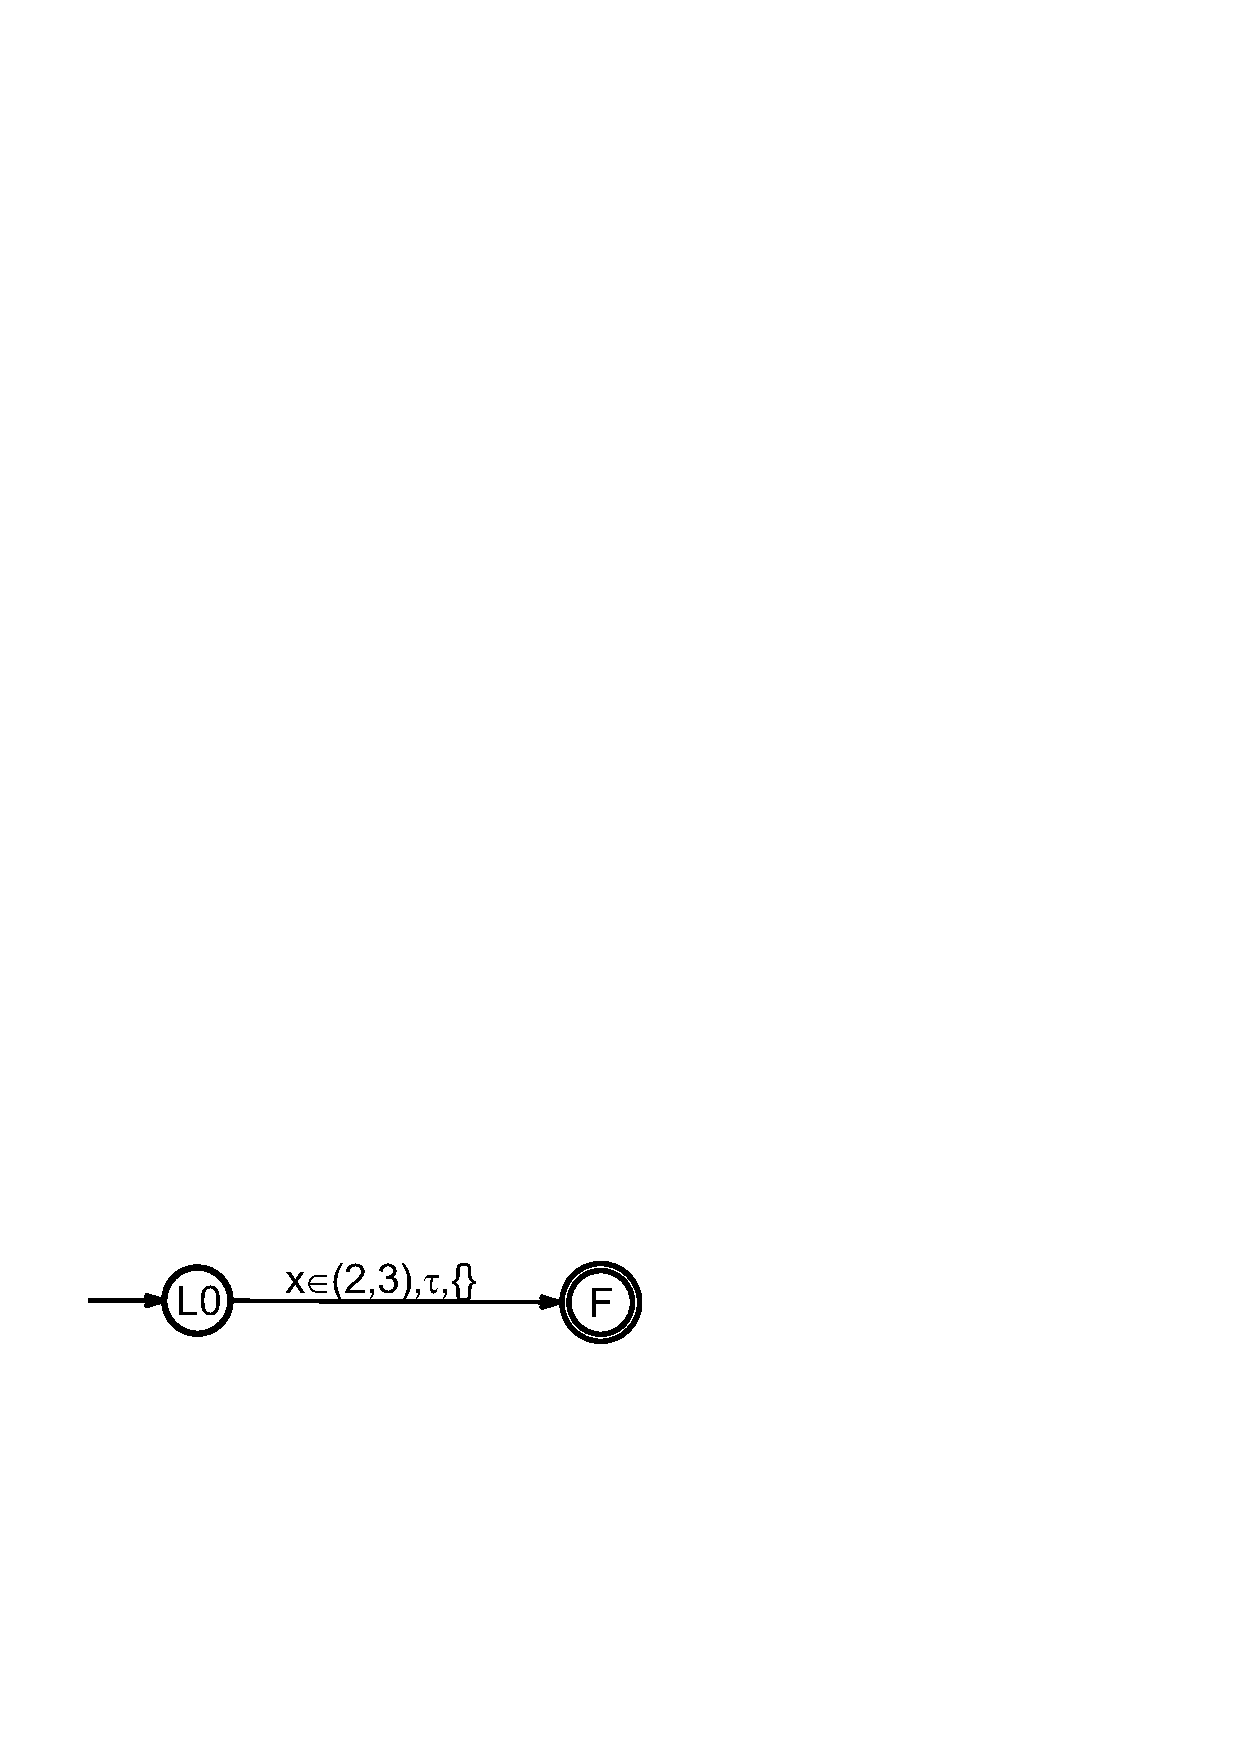
\includegraphics[scale=0.7]{open.png}
\end{figure}

%Now, consider the following run on the above timed automaton,
\begin{figure}[h!]
\centering
\includegraphics[scale=0.7]{openrun.png}
\end{figure}  
\end{proof}

\begin{theorem}
Let {\it A} = \{{\it A}\textsubscript{1},{\it A}\textsubscript{2}...,{\it A}\textsubscript{n}\} be a network of n timed automata from the class Closed Interval, with semantics (S, s\textsubscript{0},$\rightarrow$). Consider $\bar{l} \textsuperscript{1},\bar{l} \textsuperscript{2},...,\bar{l} \textsuperscript{n}  \epsilon  (L\textsubscript{1} \times L\textsubscript{2} \times...\times L\textsubscript{m})$ and valuations w\textsubscript{1} = (u\textsubscript{1},v\textsubscript{1}), w\textsubscript{2} = (u\textsubscript{2},v\textsubscript{2}),..., w\textsubscript{3} = (u\textsubscript{3},v\textsubscript{n}) such that there exists a run $R$, $(\bar{l} \textsuperscript{1},w\textsubscript{1}) \rightarrow (\bar{l} \textsuperscript{2},w\textsubscript{2}) \rightarrow ... \rightarrow (\bar{l} \textsuperscript{n},w\textsubscript{n})$. If w\textsubscript{1} is an integer evaluation then there exists integer valuations  w\textsuperscript{'}\textsubscript{1}, w\textsuperscript{'}\textsubscript{2},..., w\textsuperscript{'}\textsubscript{n} such that

\begin{equation}
(\bar{l} \textsuperscript{1},w\textsuperscript{'}\textsubscript{1}) \rightarrow (\bar{l} \textsuperscript{2},w\textsuperscript{'}\textsubscript{2}) \rightarrow ... \rightarrow (\bar{l} \textsuperscript{n},w\textsuperscript{'}\textsubscript{n})
\end{equation}

\end{theorem}
\begin{proof}
We are going to prove this by using induction on the length of run $R$.
\\
\par
w\textsuperscript{'}\textsubscript{1} = w\textsubscript{1}. It is given that w\textsubscript{1} is an integer clock valuation.
\\
%\bigskip
%\linebreak
\par
\indent Consider the k\textsuperscript{th} transition of $R$, $(\bar{l} \textsuperscript{k},w\textsubscript{k}) \rightarrow (\bar{l} \textsuperscript{k+1},w\textsubscript{k+1})$
\\Induction Step: There exists integer clock valuations w\textsuperscript{'}\textsubscript{1},...,w\textsuperscript{'}\textsubscript{k} such that $(\bar{l} \textsuperscript{1},w\textsuperscript{'}\textsubscript{1}) \rightarrow (\bar{l} \textsuperscript{2},w\textsuperscript{'}\textsubscript{2}) \rightarrow ... \rightarrow (\bar{l} \textsuperscript{k},w\textsuperscript{'}\textsubscript{k})$. $w\textsuperscript{'}\textsubscript{k}$ and $w\textsubscript{k}$ lie in the same region $R\textsubscript{k}$.  
\par
Consider the transition, $(\bar{l} \textsuperscript{k},w\textsubscript{k}) \rightarrow (\bar{l} \textsuperscript{k+1},w\textsubscript{k+1})$.
This can also be written as, $(\bar{l} \textsuperscript{k},w\textsubscript{k}) \rightarrow (\bar{l} \textsuperscript{k},\bar{w}\textsubscript{k}) \rightarrow (\bar{l} \textsuperscript{k+1},w\textsubscript{k+1})$. Here we wait for some time to reach from $w\textsubscript{k}$ to  $\bar{w}\textsubscript{k}$, $\bar{w}\textsubscript{k}\; \epsilon \; g$ and $r(\bar{w}\textsubscript{k}) = w\textsubscript{k+1}$.
\\
%We already know that $\exists\; w\textsubscript{k}$ and $\bar{w}\textsubscript{k}$ such that $(\bar{l} \textsuperscript{k},w\textsubscript{k}) \rightarrow (\bar{l} \textsuperscript{k},\bar{w}\textsubscript{k}) \rightarrow (\bar{l} \textsuperscript{k+1},w\textsubscript{k+1})$.  So, we can reach from point $w\textsubscript{k}$ in region $R\textsubscript{k}$ to $\bar{w}\textsubscript{k}$ in region $\bar{R}\textsubscript{k}$ after waiting for some time. 
From propositions in section 1.1.3, it can be inferred that $\exists$ an integer valuation $\bar{w}\textsuperscript{'}\textsubscript{k}$ in region $\bar{R}\textsubscript{k}$ such that after waiting for some time, we can reach $\bar{w}\textsuperscript{'}\textsubscript{k}$ from $w\textsuperscript{'}\textsubscript{k}$ and both $\bar{w}\textsuperscript{'}\textsubscript{k}$ and $\bar{w}\textsubscript{k}$ lie in the same region $\bar{R}\textsubscript{k}$.Also $w\textsuperscript{'}\textsubscript{k+1}$ is an integer valuation since reset operations update a clock to an integer value.  

\end{proof}



\pagebreak


%References
\addcontentsline{toc}{chapter}{References}
\bibliography{References}
%Relabels bibliography title as "References"
\renewcommand\bibname{References}
\begin{thebibliography}{9}
%Gives invariant reference tag to particular referece, use ~\cite{Each Author's Last Initial}
\bibitem{UPP2SF}
Miroslav Pajic, Insup Lee, Rahul Mangharam, Oleg Sokolsky, UPP2SF: Translating UPPAAL Models to SimulinkJournal, Universitty of Pennsylvania, Tech. Rep., Oct 2011
%Another Example
%\bibitem{TMO1}
%M. Taketani, S. Machida, and S. Onuma, Prog. Theor. Phys (Kyoto) {\bf 7} (1952) 45.
\end{thebibliography}

\end{document}
